%
%  D0018E report 1
%
%  Created by Anders Lindmark on 2012-10-31.
%  Copyright (c) 2011 Anders Lindmark. All rights reserved.
%
%\documentclass[]{article}
\documentclass[12pt, a4paper,titlepage]{article}

% Use utf-8 encoding for foreign characters
\usepackage[utf8]{inputenc}
\usepackage[english]{babel}

% Setup for fullpage use
\usepackage{fullpage}

\usepackage{float}

% Uncomment some of the following if you use the features
%
% Running Headers and footers
%\usepackage{fancyhdr}

% Multipart figures
%\usepackage{subfigure}

% More symbols
\usepackage{amsmath}
%\usepackage{amssymb}
%\usepackage{latexsym}

% Surround parts of graphics with box
\usepackage{boxedminipage}

% Package for including code in the document
\usepackage{listings}

% If you want to generate a toc for each chapter (use with book)
\usepackage{minitoc}

% This is now the recommended way for checking for PDFLaTeX:
\usepackage{ifpdf}

%\newif\ifpdf
%\ifx\pdfoutput\undefined
%\pdffalse % we are not running PDFLaTeX
%\else
%\pdfoutput=1 % we are running PDFLaTeX
%\pdftrue
%\fi

\ifpdf
\usepackage[pdftex]{graphicx}
\else
\usepackage{graphicx}
\fi

\usepackage{tikz}
\usetikzlibrary{positioning,arrows,fit,shapes,calendar,chains}

\usepackage{pgfplots}
\usepackage{pgfplotstable}

\usepackage{hyperref}

\usepackage{enumerate}

\usepackage{eso-pic}

\usepackage{color}
\definecolor{error}{RGB}{193,27,23} % #C11B17, Firebrick3
\definecolor{warning}{RGB}{229,103,23} % #E56717, Dark Orange2
\definecolor{codebg}{RGB}{245,245,245}
\definecolor{dkgreen}{rgb}{0,0.6,0}
\definecolor{poop}{rgb}{0.82,0.71,0.15}

\usepackage{parskip}
\setlength{\parskip}{0.4cm}
\setlength{\parindent}{0.6cm}

%\title{\huge\sffamily D7001D  Home examination}
%\author{Anders Lindmark, \emph{830604-8995}}
%\date{\today}

% http://tex.stackexchange.com/questions/16501/problem-with-special-characters-in-listings
%\lstset{literate=%
%{å}{{\aa}}1
%ä}{{\"a}}1
%{ö}{{\"o}}1
%{Å}{{\AA}}1
%{Ä}{{\"A}}1
%{Ö}{{\"O}}1
%}
\lstdefinelanguage{pseudo}{morekeywords={for,if,else,do,then,to,return,while,break}}
\lstset{
%backgroundcolor=\color{lightgray},
backgroundcolor=\color{codebg},
%title=\lstname,
frame=lines,
%inputencoding=utf8,
inputencoding=ansinew,
extendedchars=\true,
%basicstyle=\small,
basicstyle=\small,
commentstyle=\color{red},
numberstyle=\footnotesize,
stringstyle=\color{poop},
breaklines=true,
%keywordstyle=\color{black}\bfseries,
language=Python,
numbers=left,
}


\begin{document}
\ifpdf
\DeclareGraphicsExtensions{.pdf, .jpg, .tif}
\else
\DeclareGraphicsExtensions{.eps, .jpg}
\fi

\begin{titlepage}
\ 
\begin{center}
\vfill
{\huge\sffamily D0018E Report (1)}
\rule{\linewidth}{0.3mm}\\
Anders Lindmark \\
\vfill
\ 
\vfill
{\textbf{\today}}
\end{center}
\end{titlepage}

\tableofcontents
\newpage

\section{Establish a minimalistic website}
\subsection{Development environment}
The framework I have chosen to use is
Django\footnote{\url{https://www.djangoproject.com/}}. 
It is a framework that I have previous experience with and which I think is
very powerful aswell as easy to get started with.
It has a very good object-relational mapper (ORM) for working with databases as well
as support for running raw SQL-queries which are then mapped into objects
automatically using the ORM.

There are probably many good IDE's for developing in python/Django, NetBeans
being the one I usually use, but I will work with the editor \emph{vim}. It is the 
editor I'm most comfortable with, and vim combined with
\emph{screen}\footnote{\url{http://www.gnu.org/software/screen/}} and an
ssh-client enables me to switch computers and continue working where I left
off without having to install an IDE and download/upload code.

I will use \emph{git}\footnote{\url{http://git-scm.com/}} to keep track of code
and documentation changes which also enables me to go back to a point in
time incase I forget to document something in one of these hand-ins.

\subsection{The database}
Since I am developing on my own server I will use the 
\emph{MySQL}-installation already present on it.
I have started modelling the tables that I think I need for this application, using
the Django modelling system. When using this system you define a set of 
objects that represent the different tables and their columns. You can easily
specify relationships between the tables aswell. 

\subsubsection{Django models}
The models that I have come up with so far, and these might change in the
future when more work is done, are:

\begin{itemize}
\setlength\itemsep{-1pt}
\item Customer - A user on the site. Django has a user-system already and this
model extends that system with the extra information we need.
\begin{lstlisting}
class Customer(models.Model):
    """ 
    Contains extra information about a customer other than the fields that are available in django-auth.
    """
    # For now, store all address info in one field, i.e "Bob Bobster\n13Bob street\nBobtown"
    address = models.CharField(max_length=150) 
    phone_number = models.CharField(max_length=20)
    user = models.OneToOneField(User) # The user-field points into django's own auth-system.
\end{lstlisting}

\item Category - Different categories of products
\begin{lstlisting}
class Category(models.Model):
    """ 
    Represents a group of specific assets, i.e if we are selling food then "Snacks" could be a category
    """
    name = models.CharField(max_length=50)
    description = models.CharField(max_length=150)
\end{lstlisting}

\item Asset - The different products themselves
\begin{lstlisting}
class Asset(models.Model):
    """ 
    Represents a product.
    """
    name = models.CharField(max_length=50)
    description = models.CharField(max_length=150)
    category = models.ForeignKey(Category) # Which category does this asset belong to
    stock = models.IntegerField() # How many of this asset are in stock
\end{lstlisting}

\item Basket - The current shopping basket for a specific customer
\begin{lstlisting}
class Basket(models.Model):
    """
    Shopping basket, contains a list of assets and which customer it belongs to.
    """
    assets = models.ManyToManyField(Asset)
    customer = models.ForeignKey(Customer)
\end{lstlisting}

\item Order - A placed order
\begin{lstlisting}
class Order(models.Model):
    """
    A placed order, contains information about which assets was ordered, which customer placed the order and
    when the order was placed/shipped.
    """
    assets = models.ManyToManyField(Asset)
    customer = models.ForeignKey(Customer)
    date_placed = models.DateTimeField(auto_now=True) # Date the order was placed
    date_filled = models.DateTimeField() # Date the order was filled 
\end{lstlisting}
\end{itemize}

\subsubsection{SQL models}
Django takes the models that you have created and outputs SQL-code.
Normally this is done behind the scenes but you can get the SQL-code used
to create the tables. The code for the current version of my models looks like
this:

\lstset{language=SQL}
\begin{lstlisting}
CREATE TABLE `shopping_customer` (
    `id` integer AUTO_INCREMENT NOT NULL PRIMARY KEY,
    `address` varchar(150) NOT NULL,
    `phone_number` varchar(20) NOT NULL,
    `user_id` integer NOT NULL UNIQUE
)
;
ALTER TABLE `shopping_customer` ADD CONSTRAINT `user_id_refs_id_40cf930a` FOREIGN KEY (`user_id`) REFERENCES `auth_user` (`id`);

CREATE TABLE `shopping_category` (
    `id` integer AUTO_INCREMENT NOT NULL PRIMARY KEY,
    `name` varchar(50) NOT NULL,
    `description` varchar(150) NOT NULL
)
;
CREATE TABLE `shopping_asset` (
    `id` integer AUTO_INCREMENT NOT NULL PRIMARY KEY,
    `name` varchar(50) NOT NULL,
    `description` varchar(150) NOT NULL,
    `category_id` integer NOT NULL,
    `stock` integer NOT NULL
)
;
ALTER TABLE `shopping_asset` ADD CONSTRAINT `category_id_refs_id_71ff6d8a` FOREIGN KEY (`category_id`) REFERENCES `shopping_category` (`id`);

CREATE TABLE `shopping_basket_assets` (
    `id` integer AUTO_INCREMENT NOT NULL PRIMARY KEY,
    `basket_id` integer NOT NULL,
    `asset_id` integer NOT NULL,
    UNIQUE (`basket_id`, `asset_id`)
);
ALTER TABLE `shopping_basket_assets` ADD CONSTRAINT `asset_id_refs_id_4c78df9` FOREIGN KEY (`asset_id`) REFERENCES `shopping_asset` (`id`);

CREATE TABLE `shopping_basket` (
    `id` integer AUTO_INCREMENT NOT NULL PRIMARY KEY,
    `customer_id` integer NOT NULL
);
ALTER TABLE `shopping_basket` ADD CONSTRAINT `customer_id_refs_id_20577cdd` FOREIGN KEY (`customer_id`) REFERENCES `shopping_customer` (`id`);
ALTER TABLE `shopping_basket_assets` ADD CONSTRAINT `basket_id_refs_id_1faa067c` FOREIGN KEY (`basket_id`) REFERENCES `shopping_basket` (`id`);

CREATE TABLE `shopping_order_assets` (
    `id` integer AUTO_INCREMENT NOT NULL PRIMARY KEY,
    `order_id` integer NOT NULL,
    `asset_id` integer NOT NULL,
    UNIQUE (`order_id`, `asset_id`)
);
ALTER TABLE `shopping_order_assets` ADD CONSTRAINT `asset_id_refs_id_4d2211a4` FOREIGN KEY (`asset_id`) REFERENCES `shopping_asset` (`id`);

CREATE TABLE `shopping_order` (
    `id` integer AUTO_INCREMENT NOT NULL PRIMARY KEY,
    `customer_id` integer NOT NULL,
    `date_placed` datetime NOT NULL,
    `date_filled` datetime NOT NULL
);
ALTER TABLE `shopping_order` ADD CONSTRAINT `customer_id_refs_id_28221386` FOREIGN KEY (`customer_id`) REFERENCES `shopping_customer` (`id`);
ALTER TABLE `shopping_order_assets` ADD CONSTRAINT `order_id_refs_id_29c844c0` FOREIGN KEY (`order_id`) REFERENCES `shopping_order` (`id`);
\end{lstlisting} 
Here you can also see how it adds relationships between the tables.

\subsection{The website}
I would like to prefix this part by stating that I am not a good designer,
so the webpage that you see might make your eyes hurt a bit.

\subsubsection{Tools}
At its current state, the website uses HTML, CSS and JavaScript. 
I am using JQuery\footnote{\url{http://jquery.com/}} as the JavaScript-library
because I have previous experience with it and it makes things alot easier and
more convenient when developing and has good tools for using AJAX.

\subsubsection{The result}

I have created a very basic skeleton of a website that I think has all the pieces
I need for this application. I started by thinking about what components are
needed. I came up with this list:
\begin{description}
\setlength\itemsep{-5pt}
\item[Header] A place to put the logo of the webshop
\item[Footer] A place to end the webpage and put short, basic, information
		about it
\item[Navigation] A place to put global links, such as ``My Account'' and ``Shopping basket''.
\item[Body] The body needs two components, two columns, where the first
	column is a category-list and the second column is the main content page.
	The main content page contains information about the current product
	or the shopping basket, etc.
\end{description}

I also wanted you to be able to see the contents of the shopping basket at a
glance, my current solution for this is hovering the mouse over the shopping
basket link which toggles the visibility of a \emph{\lstinline{<div>}}-container.
In the future this will be done using an ajax call.

The website in it's current state can be seen here: \url{http://localghost.net/d0018e/1/}. 
A small screenshot can be seen in figure \ref{fig:sshot}.
\begin{figure}
\centering
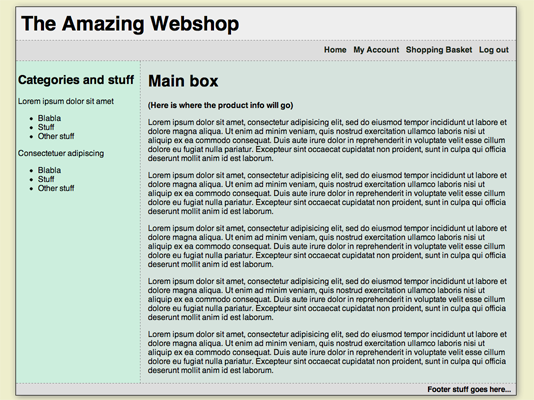
\includegraphics[width=10cm]{Screenshot_2012-11-16.png}
\caption{Screenshot of the webpage on November 16, 2012}
\label{fig:sshot}
\end{figure}

\subsubsection{References}
I used this guide:
\url{http://www.456bereastreet.com/lab/developing_with_web_standards/csslayout/2-col/}
when creating the website, it shows how to do a simple two-column webpage.

I used the CSS-information on \url{http://www.w3schools.com/} as a reference.

JQuery has excellent documentation available on \url{http://docs.jquery.com/}
and for positioning the shopping-basket information I used this addon: 
\url{http://docs.jquery.com/UI/API/1.8/Position}

\subsubsection{To be done}
Because Django uses a template system to render the HTML I need to 
convert my webpage into this format. 
This will not require alot of work since the template language is plain 
HTML with special tags added for Django-logic.
The django template system has the benefit being able to specify a base page
which contains global information such as header and footer and then
specifying ``blocks'' that are filled in dynamically for each subpage.


\section{Content management system}
The basic point of a CMS is to separate the administration of the website and
the editing of webpage code from the content. This allows users to edit the
webpage while focusing on the content and not the other details surrounding
a large site, especially the details of editing html and styling the content.



\end{document}
